\documentclass[12pt]{amsart}
\usepackage{amsaddr}
\usepackage[draft]{../marktext} 
%% Remove draft for real article, put twocolumn for two columns
\usepackage[draft]{../svmacro}
\usepackage[utf8]{inputenc}
\usepackage[style=alphabetic, backend=biber]{biblatex}
\addbibresource{bibliography.bib}

%% commentary bubble
\newcommand{\SV}[2][]{\sidenote[colback=green!10]{\textbf{SV\xspace #1:} #2}}

%% Title 
\title{ Worksheet 2 }
\author{MATH 101}
\address{Fulbright University, Ho Chi Minh City, Vietnam}

%\author{Co-author}
%\address{  }
%\email {  }
%
\date{\today}

\begin{document}

\maketitle

\begin{question}
	Consider the following graph of a function $y = f(x)$.
	\begin{center}
		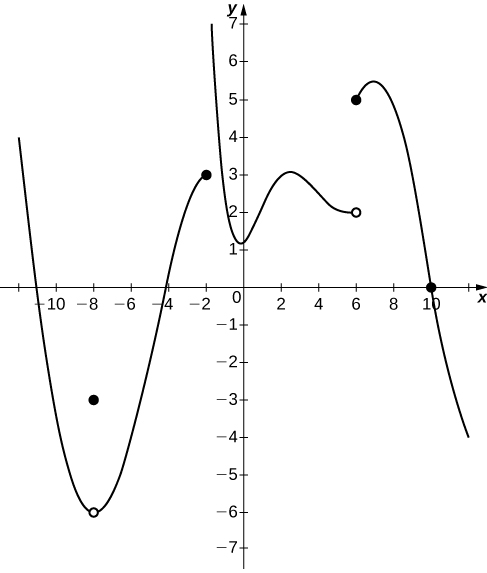
\includegraphics[width=0.45\textwidth]{figures/1.jpeg}
	\end{center}
	True or False?
	\begin{enumerate}
		\item $\displaystyle \lim_{x\to 10} f(x)=0$
		\item $\displaystyle \lim_{x \to -2^+} f(x) = 3$
		\item $\displaystyle \lim_{x \to -8} f(x) = f(-8)$
		\item $\displaystyle \lim_{x \to 6} f(x) = 5 $
	\end{enumerate}

\end{question}


\begin{question}
	What is the limit of the following?
	If the limit DNE, please specify left and right limits.
	\begin{enumerate}
		\item $\lim_{x\to a} \frac{1}{(x -a)^n}$ where $n$ is odd.
		      \vspace{5cm}
		\item $\lim_{x\to a} \frac{1}{(x -a)^n}$ where $n$ is even.
		      \vspace{5cm}
		\item $\lim_{x \to 2} \frac{x^2 - 4}{x-2}$
		      \vspace{5cm}
		\item $\lim_{x \to 2} \frac{|x^2 - 4|}{x-2}$
		      \vspace{5cm}
	\end{enumerate}
\end{question}


\begin{theorem}
	The following are VERY important limit laws.
	The proof of them is out of the scope of this class but I will
	tell you if you come to office hours.

	Suppose $\lim_{x\to a} f(x) = L$ and $\lim_{x\to a} g(x) = M$.
	Then,
	\begin{enumerate}
		\item $\displaystyle \lim_{x\to a} (f(x) + g(x)) =$
		\item $\displaystyle \lim_{x\to a} (f(x) - g(x)) =$
		\item $\displaystyle \lim_{x\to a} (f(x) \cdot g(x)) =$
		\item $\displaystyle \lim_{x\to a} \frac{f(x)}{g(x)} =$
		\item $\displaystyle \lim_{x\to a} (f(x))^n =$
		\item $\displaystyle \lim_{x\to a} (f(x))^{1/n} =$
	\end{enumerate}

\end{theorem}


\begin{question}
	Find the limit
	\begin{enumerate}
		\item $\displaystyle \lim_{x\to a} x = $
		\item $\displaystyle \lim_{x\to a} c = $
		\item $\displaystyle \lim_{x\to a} (2x -1)\sqrt{x + 4} = $
	\end{enumerate}
\end{question}

\begin{question}
	Graph the function
	\begin{equation*}
		g(x) = \begin{dcases}
			x^3 - 1 \,, & x \leq 2  \\
			1 \,,       & x > 2 \,.
		\end{dcases}
	\end{equation*}
	Find
	\begin{equation*}
		\lim_{x\to 2} g(x)
	\end{equation*}

\end{question}

\begin{question}
	What is a polynomial function?
\end{question}
\begin{theorem}
	Let $p(x)$ and $q(x)$ be polynomial functions. Then,
	\begin{equation*}
		\lim_{x \to a} p(x) = \,.
	\end{equation*}
\end{theorem}

\begin{question}
	Find the following limits.
	\begin{enumerate}
		\item $\displaystyle\lim_{x \to 4}  \frac{ x^2 - 16}{x - 4}$
		\item $\displaystyle\lim_{h \to 0}  \frac{ (1 + h)^2 - 1}{h}$
		\item $\displaystyle\lim_{x \to 1/2}  \frac{ 2x^2 + 3x - 2}{2x -1}$
	\end{enumerate}
\end{question}

\begin{theorem}[Squeeze Theorem]
	Let \( f(x) \), \( g(x) \), and \( h(x) \) be functions defined for all \( x \neq a \) over an open interval containing \( a \). Suppose:

	\[
		f(x) \leq g(x) \leq h(x) \quad \text{for all } x \neq a \text{ in an open interval containing } a
	\]

	and

	\[
		\lim_{x \to a} f(x) = L = \lim_{x \to a} h(x)
	\]

	where \( L \) is a real number. Then,

	\[
		\lim_{x \to a} g(x) = L.
	\]
\end{theorem}

\begin{question}
	We know from our discussion in the last class that
	\begin{equation*}
		\lim_{x \to 0} \sin \left( \frac{1}{x} \right) = DNE \,.
	\end{equation*}
	What is it still the same with
	\begin{equation*}
		\lim_{x \to 0} x \sin \left( \frac{1}{x} \right) ?\,.
	\end{equation*}
\end{question}

\begin{question}
	Discuss
	\begin{enumerate}
		\item Formula (2.18) in Section 2.3
		\item Example 2.25
		\item Checkpoint 2.20
	\end{enumerate}

\end{question}


\printbibliography
%\bibliography{refs}
%\bibliographystyle{halpha-abbrv}


\end{document}
